\chapter{\label{konzept}Ressourcenbeschr"ankung}
%--Ressourecnbeschr"ankung ??
Dieses Kapitel beschreibt die Modellierung von Ressourcenbeschr"ankungen in der Infiniband
Simulation. Zun"achst soll jedoch gekl"art werden, was unter
Ressourcenbeschr"ankung zu verstehen ist.

Bei der konkreten Implementierung eines Systems, z.\,B. 
Infiniband-Controller, werden ausf"uhrende Einheiten ben"otigt,
z.\,B. Prozessoren oder spezielle Hardware (DSP, ASIC, ASIP).  Selbst ein rein
in Software geschriebenes System ben"otigt mindestens einen Prozessor zur
Ausf"uhrung. Die Anzahl solcher ausf"uhrenden Einheiten ist im Allgemeinen
endlich, anders ausgedr"uckt: Die Zahl der Ressourcen ist
beschr"ankt. Eine Beschr"ankung von Betriebsmitteln wie Speicher oder
E/A-Peripherie soll nicht Gegenstand der Diskussion sein. 


Den ausf"uhrenden Einheiten (Ressourcen) stehen auszuf"uhrende Einheiten
(Prozesse, Tasks)\footnote{Die Begriffe \emph{Prozess}, \emph{Task} oder
  \emph{Aufgabe} werden in dieser Arbeit synonym, als Bezeichnung f"ur
  T"atigkeiten, verwendet.}  gegen"uber. Notwendigerweise ben"otigt
jeder Prozess eine Ressource zur Ausf"uhrung. Es besteht jedoch die
M"oglichkeit das ein Prozess auf unterschiedlichen Ressourcen ausgef"uhrt
werden k"onnte. Dieser Zusammenhang ist in Abbildung \ref{fig:ib_spec_graph}
dargestellt. Die formale Grundlage f"ur diese Modellierungsform ist in den 
Arbeiten \cite{btt:1998, teich:1997} beschrieben. Folgende Begrifflichkeiten 
werden dabei verwendet:
\begin{description}
\item[Problemgraph:] Ein gerichteter Graph $G_P = (V_P,E_P)$ mit Knotenmenge $V_P$ 
und Kantenmenge $E_P$. Knoten repr"asentieren funktionale Aufgaben sowie 
Kommunikationsaufgaben. Kanten stellen gerichtete Datenabh"angigkeiten dar.
\item[Architekturgraph:] Ein gerichteter Graph $G_A = (V_A,E_A)$ mit der 
Menge der allozierbaren Komponenten $V_A$ und der Menge der gerichteten 
Kommunikationsverbindungen $E_A$.
\item[Spezifikationsgraph:] Der gerichtete Spezifikationsgraph $G_S = (V_S,E_S)$ besteht aus einem Problemgraphen $G_P = (V_P,E_P)$ und einem Architekturgraphen $G_A = (V_A,E_A)$ und Abbildungskanten $E_M$ mit $V_S = V_P \cup V_A$ und $E_S = E_P \cup E_A \cup E_M$.
\end{description}
Diese Art der Modellierung erm"oglicht es, ein Verhalten unabh"angig von der zu 
verwendenden Architektur zu beschreiben. Ausgehend von einer Spezifikation k"onnen 
unterschiedliche Implementierungen entstehen, welche sich in der \emph{Allokation}
(Auswahl der verwendeten Architekturknoten) und in der \emph{Bindung} von Problemknoten auf 
Architekturknoten unterscheiden. Dadurch ergeben sich unterschiedliche Bewertungen f"ur 
unterschiedliche Implementierungen. Beispielhaft seien hier Chipfl"ache, 
Latenz und Stromverbrauch genannt. F"ur die Entscheidung welche konkrete
Implementierung verwendet werden soll, kann ein Optimierungsverfahren 
eingesetzt werden.

\begin{figure}
\begin{center}
\includegraphics[width=12cm]{ib_spec_graph}
\caption{Spezifikationsgraph: Prozesse aus dem Problemgraphen ($G_P$)
werden mittels Abbildungskanten ($E_M$) auf die Ressourcen des
Architekturgraphen ($G_A$) abgebildet.}
\label{fig:ib_spec_graph}
\end{center}
\end{figure} 

Die Leistungsbewertung einer allgemeinen Implementierung ist
nicht trivial. Hierf"ur 
eignen sich am besten simulative Verfahren zur Average-Case-Bewertung.
Also eine direkte Simulation oder ein Trace-Driven-Simulation 
Verfahren \cite{lrd:2001}. F"ur die Simulation des Infinband-HCA
 wird ein Simulationsframework verwendet, mit dem die 
Ressourcenbeschr"ankung nachgestellt werden kann. Dieses 
tr"agt den Name \emph{Virtual-Processing-Components}-Framework 
(\emph{VPC}-Framework) und wird im Folgenden erl"autert.
%TODO zitat

\section{VPC-Framework}


Ein VPC-Simulator unterscheidet sich wesentlich von "ublichen
Befehlssatzsimulatoren oder zyklenakkuraten Simulatoren. Bei diesen wird ein
Programm auf der simulierten Architektur ausgef"uhrt. Der Simulator bildet
dabei eine reale Hardwarekomponente m"oglichst detailgetreu nach. Derartige
Simulationen sind aufwendig und bieten sich daher nicht f"ur die Simulation komplexer
Systeme an. Eine Simulation auf System\-ebene ben"otigt entsprechende Einheiten
mit gr"oberer Granularit"at. Als Einheiten bieten sich hier zum Beispiel Prozesse
an. Da diese jedoch sehr komplexe Aufgaben darstellen, w"urde nun wiederum der
Umfang des Simulators explodieren.


Alternativ wird ein System zur Simulation durch entsprechend abstraktere Modelle
dargestellt. Beispiele hierf"ur sind Petri-Netze\cite{baumgarten:1990}, 
Zustandsautomaten\cite{harel:1987} oder der
oben vorgestellte Problemgraph. Ein solches Modell beschreibt eine Komposition
von Prozessen. Da Implementierungsdetails der Prozesse dabei nicht
betrachtet werden, ist das Zusammenspiel und Zeitverhalten der Prozesse Gegenstand der
Simulation. Dabei geht der Bezug zur Architektur (z.\,B. Hardwarekomponenten) %%todo
 verloren. 


Das VPC-Simulationsmodell beh"alt die Trennung von Architektur und Problem
bei. Abbildung \ref{fig:vpc-framework-ueberblick} zeigt eine schematische
Darstellung des Simulationsframeworks. Das Problem wird mit Hilfe von
SystemC-Sprachkonstrukten modelliert. Die Komponenten der Architektur werden
durch virtuelle Komponenten, welche als Objekte in C++ implementiert sind,
dargestellt. Diese virtuellen Komponenten bilden den Kern der Zeitmodellierung im
Simulationsframework. Durch die Mehrzahl von Komponenten
und Prozessen muss eine  Multitasking- und Multiprozessorarchitektur durch das
Framework betrachtet werden. Weiterhin sind die Komponenten durch eigene
Ablaufplanungsstrategien, die simuliert werden m"ussen, gekennzeichnet.

\begin{figure}
\begin{center}
\includegraphics[width=12cm]{ib_vpc_framework}
\caption{Schema des VPC-Simulations-Framework. Tasks werden "uber einen
  zentralen Direktor den ausf"uhrenden Komponenten zugeordnet. Den einzelnen
  virtuellen Komponenten (VPC) k"onnen unterschiedliche Schedulingstrategien
  zugeordnet werden.}
\label{fig:vpc-framework-ueberblick}
\end{center}
\end{figure}

F"ur die Simulation des Infiniband-HCA wurde dieses in 17 separate Prozesse 
zerlegt (vgl. Abbildung \ref{fig:hca_func_units_lib} auf Seite 
\pageref{fig:hca_func_units_lib}). Jeder dieser Prozesse
 stellt einen Problemgraphknoten dar.

Ein objektorientiertes Modell soll die Architektur f"ur die Simulation
  abbilden. Jede Komponente\footnote{Knoten des
  Architekturgraphen} wird durch ein eigenes Objekt repr"asentiert. Ein
  \module{Scheduler}-Objekt wird einer Komponente zugeordnet und stellt die
  Ablaufplanung sicher. Eine zentrale Instanz zur Verwaltung (der Direktor)
  "ubernimmt die Aufgaben \emph{Bindung} und \emph{Allokation} der 
Komponenten. Eine
"Ubersicht findet sich im UML-Klassendiagramm in Abbildung
\ref{fig:vpcframework}.
\begin{figure}
\begin{center}
\includegraphics[width=14cm]{vpc-framework}
\caption{UML-Klassendiagramm des VPC-Frameworks.}
\label{fig:vpcframework}
\end{center}
\end{figure}
\subsection{Component}
Die \module{Component} ist die Zentrale Einheit des
Virtual-Processing-Components-Frameworks. Daher folgt auch der Name des
Frameworks. 


Eine Komponente stellt die ausf"uhrende Umgebung f"ur ein Prozess dar. Einen
Prozess an eine Ressource zu binden, f"uhrt zu unterschiedlichen Kosten oder
Bewertungen. F"ur die Systemsimulation sind
die Ausf"uhrungszeiten der Prozesse und somit die Latenz des Problems die
wichtigste Zielfunktion. Die Bindung eines Tasks an eine Komponente zieht also
unterschiedliche Ausf"uhrungszeiten und somit unterschiedliche Latenz nach 
sich.\footnote{Die einzelnen Ausf"uhrungszeiten eines Prozesses muss f"ur alle 
zur Ausf"uhrung in Frage kommenden Ressourcen bekannt sein, 
z.\,B. durch Sch"atzung.}

Die Ausf"uhrung eines Prozesses auf einer Ressource wird als eine funktional 
atomare Operation angesehen. Unterbrechungen durch Multitasking f"uhren nicht
zu unterschiedlichem Verhalten sondern nur zu verschiedenen Antwortzeiten der 
Prozesse. Dieses prozessakurate Simulationskonzept erm"oglicht einen geringen 
Simulationsaufwand, trotzdem sind die Auswirkungen von Ressourcenbeschr"ankung 
und Schedulingstrategien auf die Latenz simulierbar. Dazu m"ussen den einzelnen 
Prozessen im Simulationsmodell Ausf"uhrungszeiten zugewiesen
werden. Erst nach Ablauf dieser Zeit stehen die Ausgangsdaten der Berechnung
bereit und folgende Module k"onnen aktiviert werden. SystemC bietet mit 
der \code{wait}-Funktion ein m"achtiges Konzept zur Zeitmodellierung 
\cite{glms:2002}. Dieser Funktion wird die abzuwartende \emph{delay}-Zeit
"ubergeben. 



%%%todo
Unterschiedliche \emph{delay}-Zeiten werden wie folgt modelliert 
(vgl. Abbildung \ref{fig:task-component-compute}):
\begin{figure}
\begin{center}
\includegraphics[width=14cm]{task-component-compute}
\caption{Ausf"uhrungszeit in Abh"angigkeit zur ausf"uhrenden Komponente. Die
  Ausf"uhrung von Task T2 auf Komponente 2 verursacht eine Ausf"uhrungszeit von
  20 ns.}
\label{fig:task-component-compute}
\end{center}
\end{figure}
Einem Prozess wird eine \module{Component}, analog zur Bindung,
zugewiesen. Die \module{Component} besitzt eine Schnittstelle, die
\code{compute}-Funktion, f"ur den Zugriff von au"sen. Das aufrufende
Problem-Modul "ubergibt der Funktion eine eindeutige Identifikation (numerisch
oder alphanumerisch). Durch den Aufruf von \code{wait} wird die dem Prozess
zugeordnete Wartezeit abgewartet. Anschlie"send kehrt die
\code{compute}-Funktion mit \code{return} zur"uck und das Problem-Modul kann
die Berechnung fertig stellen. 


\subsection{Director}


Zur Bindung der Tasks auf die Ressourcen wird ein weiteres Objekt, der
\module{Director} verwendet. Wie ein Direktor im realen Leben ist er mit den
wesentlichen administrativen Aufgaben betreut. Der \module{Director} ist als
\emph{Singleton}-Entwurfsmuster realisiert. Also existiert nur eine Instanz
dieser Klasse.  Diese Instanz kann "uber die statische Funktion
\code{getInstance} abgerufen werden (vgl. Abbildung
\ref{fig:director_getinstance}). Nun kann die ausf"uhrende
\begin{figure}
\begin{center}
\includegraphics[width=10cm]{director_getinstance}
\caption{\module{Director} als \emph{Singleton}-Entwurfsmuster. F"ur den Zugriff
  auf die Singleton-Instanz wird eine statische Funktion bereitgestellt.}
\label{fig:director_getinstance}
\end{center}
\end{figure}
\module{Component} durch Aufruf von \code{getResource} auf dem
\module{Director}-Objekt ermittelt werden. Dabei muss eine Identifikation des
Problem-Moduls stattfinden. Es liegt nahe, diese analog zu der Identifikation
der \code{compute}-Funktion in der \module{Component} zu gestalten. Der gesamte
Mechanismus erm"oglicht sowohl statische als auch dynamische Bindung der
Prozesse an die Komponenten. Nachdem Aufruf der \code{getResource} Funktion
steht die Bindung f"ur den aufrufenden Prozess fest. Eine
\emph{Migration} von Prozessen d.\,h., das Unterbrechen eines Prozesses auf einer Ressource
und fortsetzten auf einer Anderen ist nicht m"oglich. Bei einer erneuten
Aktivierung eines Prozesses ist sehr wohl eine andere Bindung m"oglich. 

Die zu verwendende Allokation und Bindung f"ur eine Simulation wir in Form
einer Konfigurationsdatei vorgegeben. Eine Konfiguration besteht aus zwei 
Teilen, der Allokation gefolgt von der Bindung. Die Allokation wird durch 
das Schl"usselwort \code{component:} eingeleitet, gefolgt durch den Namen 
der Komponente und den zu verwendenden Scheduler. Der Scheduler kann dabei
weitere Parameter enthalten. Eine Bindung setzt sich aus dem Namen des 
Prozesses, der zu verwendenden Komponente, der Ausf"uhrungszeit in Nanosekunden und der 
Priorit"at\footnote{Wird nur f"ur priorit"atsbasietes Scheduling 
ausgewertet.} des Prozesses. Als Trennzeichen werden ein oder 
mehr \emph{Whitespaces} erwartet. Ein Beispiel:\\
\begin{verbatim}
component:  HWM1  FCFS
component:  HWM2  RoundRobin:timeslice-200ns
...
sim_mod.h_hca.qpc_manager       HWM1 4000 50
sim_mod.h_hca.h_transmit_queue  HWM2 2000 50
sim_mod.h_hca.h_send_port       HWM1 1000 50
...
\end{verbatim}
In der Zukunft soll diese Format durch ein 
universelleres XML-Format ersetzt werden.




\subsection{Scheduler}\label{scheduler}
Im Spezifikationsgraph stellen die Problemknoten die
Aktivit"atstr"ager dar. Ressourcen sind durch
Architekturknoten modelliert. Diese Grundlage ergibt eine
Mehrprozessorarchitektur. Unter der Annahme, dass ein Prozess w"ahrend seiner Laufzeit nicht von einer
Ressource zu einer anderen verschoben wird, l"asst sich der Spezifikationsgraph durch
mehrere Einprozessorarchitekturen darstellen.\footnote{Diese Annahme trifft
  hier zu, da Prozesse die atomaren Ausf"uhrungseinheiten darstellen.} Alle
aktivierten Prozesse beginnen mit der Ausf"uhrung, die im Sinne der 
simulierten (SystemC) Zeit instantan und nebenl"aufig stattfindet. Durch den
Aufruf der \code{compute}-Funktion auf der zugewiesenen Komponente wird die
verbrauchte Zeit simuliert. Rufen mehrere Prozesse auf einer \module{Component}
die \code{compute}-Funktion auf, ist es Aufgabe des \module{Schedulers}, eine
Ablaufplanung f"ur die Prozesse sicherzustellen.

Wird ein Prozess auf einer Komponente ausgef"uhrt, so ist eine Blockade des
Prozesses auszuschlie"sen.\footnote{Ebenfalls wegen der Atomarit"at der Prozesse.} Daher
 vereinfacht sich das Zustandsmodell aus Sicht
der Komponente auf die zwei Zust"ande \emph{Bereit} und
\emph{Rechnend}. Zusammen mit dem Berechnungsmodell des Problemgraphen ergibt
sich das hierarchische Thread-Zustands\-modell aus Abbildung
\ref{fig:vpc-zustandsmodell}.
\begin{figure}
\begin{center}
\includegraphics[width=10cm]{vpc-zustandmodell}
\caption{Thread-Zustandsmodell des VPC-Simulators.}
\label{fig:vpc-zustandsmodell}
\end{center}
\end{figure}

Die beiden grau hinterlegten Zust"ande unterscheiden blockierte von
nicht-blockierten Prozessen. Also solche Prozesse, die auf ihre
Vorg"angerprozesse blockiert sind und jene, die gerade auf einer Komponente
\code{compute} aufrufen. Somit ist das Ereignis \msg{ready} "aquivalent zum
Aufruf von \code{compute} und das Beenden der Funktion mit \code{return}
stellt das Ereignis \msg{block} dar. Die Unterscheidung zwischen
\emph{Rechnend}- und \emph{Bereit}-Zust"anden auf einer Komponente ist Aufgabe
des \module{Schedulers}. 



Die Nebenl"aufigkeit der Problemgraphprozesse
f"uhrt zu mehrfachen parallelen Aufrufen der \code{compute}-Funktion einer
Komponente durch unterschiedliche Prozesse. Daher existieren mehrere
Instanzen der Funktion, der Sequenzgraph in Abbildung
\ref{fig:sequenzgraph-compute} stellt dies dar.
\begin{figure}
\begin{center}
\includegraphics[width=8cm]{sequenzgraph-compute}
\caption{Mehrere Aufrufe f"uhren zu mehreren Instanzen der \texttt{compute}-Funktion.}
\label{fig:sequenzgraph-compute}
\end{center}
\end{figure}
Dabei handelt es sich um quasi-parallele Ausf"uhrung\footnote{Jede dieser Instanzen
ist dem Kontext des aufrufenden Problemknoten zugeordnet.}, die Umschaltung erfolgt
durch das SystemC-Modell. Diese Parallelit�t  erm�glicht letztendlich die Simulation
von Ablaufplannungsstrategien. Eine detaillierte Beschreibung bez�glich der
Scheduling-Simulation findet sich in \cite{vpc:2005}.

%%todo

Der durch die Simulation entstandene Ablaufplan wird aufgezeichnet und 
kann mit Hilfe von Wave-Form-Viewern visualisiert werden.\footnote{Die 
Aufzeichnung erfolgt im \emph{VCD}-Format (\emph{Value Change Dump}).}
Dabei wird f�r jede Ressource eine Datei ereugt, z.\,B.
\file{HCA1-HWM1.vcd}. Ein Signal, in solch einer Datei, repr�sentiert 
einen Prozess, welcher auf der entsprechenden Ressource gebunden ist. 
Der Typ des Signals ist \code{char}, wobei die Zeichen 'R', 'w', 'b'
die Zust�nde \emph{Rechnend}, \emph{Bereit}, \emph{Blockiert} 
repr�sentieren. Ein Beispiel eines
Ablaufplans f"ur die Infiniband Simulation zeigt Abbildung \ref{fig:trace}

\begin{figure}
\begin{center}
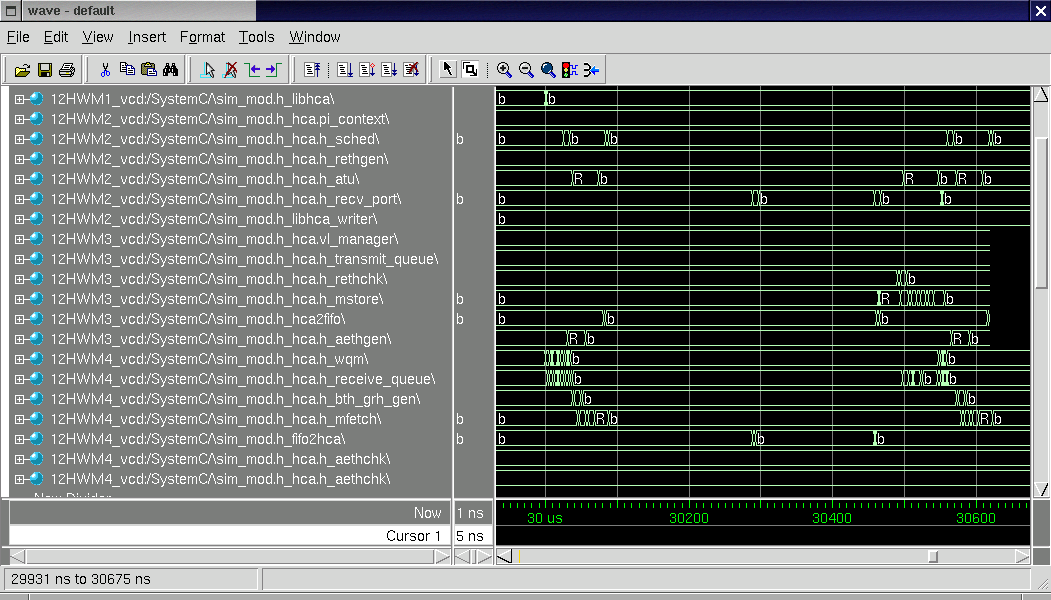
\includegraphics[width=14cm]{infiniband-mixed-mixed-trace}
\caption{\emph{Trace file} der Infiniband HCA Simulation unter Einsatz von vier Komponenten.}%%TODO verbessern
\label{fig:trace}
\end{center}
\end{figure}


\section{Simulator-Synchronisation}
Die vorgestellten Mechanismen dienen dazu jedem Prozess eine 
Ausf"uhrungszeit in Abh"angigkeit zur Bindung und Schedulingstrategie 
zuzuordnen. Auch wurde erw"ahnt das f"ur die Zeitmodellierung die 
Mechanismen von SystemC verwendet werden. Die Auftrennung in zwei 
kommunizierende Infiniband-HCA Simulationen, wie in Kapitel 
\ref{cha:ib_sim_model} vorgestellt, erweist sich jedoch als Problem
f"ur die ereignisorientierte Zeitsimulation. Der folgende Abschnitt
wird diese Problem erl"autern und die implementierte L"osung 
vorstellen. Zun"achst wird das Prinzip der ereignisorientierten Simulation
erl"autert.

%%\subsubsection{Ereignisorientierte Simulation}
Die ereignisorientierte Simulation ist dadurch gekennzeichnet, dass der
Simulator nur dann in Aktion tritt, wenn eine "Anderung (Event) stattgefunden hat. Anstatt
sich von Zeitschritt $i$ zu Zeitschritt $i+1$ zu hangeln, springt der   %%todo hangeln?????????
Simulator von einem Event zum (im Zeitverlauf) n"achsten Event. Gleichzeitig
schreitet die simulierte Zeit um diese Differenz voran. Folglich kann die
Zeitaufl"osung gro"s gew"ahlt werden, ohne zus"atzliche Aktivierungen des
Simulators auszul"osen. Beispiele f"ur ereignisorientierte Simulation finden 
sich z.\,B. bei der Simulation von VHDL- oder SystemC-Code \cite{glms:2002, sysc1}. 

Eine Liste mit offenen (noch nicht bearbeiteten) Ereignissen ist das Zentrum der
ereignisgetriebenen Simulation. Das Ereignis, welches am n"achsten in der Zukunft
liegt, wird ausgew"ahlt, abgearbeitet und die Simulationszeit wird
aktualisiert. Bei der Abarbeitung des Vorgangs (Prozesses), welches dem Event
zugeordnet ist, k"onnen neue Ereignisse samt Auftrittszeitpunkt generiert und
in die Ereignisliste eingetragen werden. Soll aufgrund einer Aktivit"at ein weiterer
Vorgang zum gleichen Zeitpunkt aktiviert werden, wird ein entsprechendes Event
mit gleichem Zeitindex generiert. Derartig erzeugte Ereignisse werden in
unterschiedlichen \emph{Delta-Zyklen} abgearbeitet. Somit wird die mehrfache
Aktivierung eines Events zum gleichen Zeitpunkt, aber in unterschiedlichen
Delta-Zyklen m"oglich. Ein zu h"aufiges Auftreten von Ereignissen kann die
Simulation nachteilig beeinflussen. Bei der zeitorientierten Simulation wird
jeder kleinste Zeitschritt nur einmal bewertet, die Delta-Zyklen der
ereignisorientierten Simulation machen unter
Umst"anden eine mehrfache Betrachtung des gleichen Zeitpunkts notwendig.

Dieses Simulationskonzept f"uhrt dazu das die Zeit nicht Schritt f"ur Schritt
voranschreitet sondern in verschieden gro"sen Schritten. Bei dem Zusammenschalten der
beiden Infiniband-HCA-Simulatoren w"urde jede Simulatorinstanz nur ihre eigene 
Zeitlinie betrachten. Wenn ein Simulator ein Datenpaket zu einem Zeitpunkt an den
anderen Simulator schickt ist nicht gew"ahrleistet das es dort zum gleichen Zeitpunkt
ankommt. Sollte die Sendezeit in der Zukunft liegen, w"are dieses Problem durch 
warten auf der Empfangsseite zu l"osen. Liegt die Sendezeit dagegen in der Vergangenheit
des empfangenden Simulators kann die Zeit nicht zur"uckgedreht werden.

Folgendes Beispiel soll die Problematik verdeutlichen: Simulator HCA-1 und Simulator HCA-2 
starten zum gleichen Zeitpunkt, sowohl gleiche Simulationszeit, als auch gleiche 
Ausf"uhrungszeit. Einer der beiden, in diesem Fall HCA-1, soll eine Reihe von Anfragen
abarbeiten, dabei werden Datenpakete erzeugt und zum HCA-2 gesendet. HCA-2 hat 
gerade nichts  zu tun sondern soll erst zu einem sp"ateren Zeitpunkt eine Consumer-Anfrage
abarbeiten. Die ereignisgesteuerte Simulation sorgt daf"ur das zu dem 
Zeitpunkt vorw"arts gesprungen wird, an dem weiter gearbeitet werden kann. Wegen der 
starken Aktivit"at im HCA-1 wird die Zeit nur in kleinen Schritten, gefolgt 
von Simulatoraktivit"at, weitergeschaltet. Im HCA-2 findet ein gro"ser Sprung
in die Zukunft statt. Nun erzeugt der HCA-1 nach einigen Berechnungsschritten 
ein Datenpaket f"ur den HCA-2, diese kommt dort jedoch in der Vergangenheit an.

Diese Problem resultiert aus der verteilten \emph{Event-Queue} der getrennten
Simulatoren. M"ogliche L"osungsans"atz sind:
\begin{itemize}
\item Keine Trennung der beiden Simulationen. (Gemeisame Event-Queue) 
\item Anpassung des SystemC Quellcodes um verteilte Event-Queues zu unterst"utzen.
\item Aufgabe der Ereignisorientierten Simulation.
\end{itemize}

Die Trennung der Simulation in zwei Instanzen erm"oglicht Tests "uber Rechnergrenzen
hinweg. Und somit auch die M"oglichkeit einen Simulator gegen eine Hardwareimplementierung
zu testen. Eine gemeinsame Simulation w"urde diese Eigenschaften zerst"oren. 

Eine Anpassung der SystemC-Bibliothek ben"otigt einen direkten Eingriff in den 
Quellcode. Dies f"uhrt zur Inkompatibilit"at der Infiniband-Simulation mit anderen 
SystemC-Installationen. Das Kosten-Nutzen Verh"altniss steht dann, auch 
wegen dem Implementierungsaufwand, in einem nicht tragbaren Verh"altnis.

Bleibt als letzte L"osung die Aufgabe der ereignisorientierten 
Simulation: In jeder Simulation l"auft ein Prozess der in einem festen 
Simulationszeitintervall die Simulationen synchronisiert. Um das auseinanderdriften
zu verhindern sollte diese Intervall m"oglichst klein sein. Eine solche Umsetzung 
hat nun wiederum den Effekt, dass die Vorteile der ereignisorientierten  
Simulation verloren gehen. Zus"atzlich kombiniert man die Nachteile von 
ereignisorientierter und zeitorientierter Simulation. Wegen der Synchronisation 
wird jeder Zeitschritt simuliert und wegen der zu Grunde liegenden ereignisorientierten
Simulation, bleibt die mehrfache Betrachtung des selben Zeitschrittes in verschiedenen
Delta-Zyklen erhalten.



Diese Nachteile k"onnen abgeschw"acht werden, wenn f"ur die Kommunikation zwischen
den Infiniband-HCA-Simulatoren eine Verz"ogerungszeit angenommen wird. Diese Implementierte
Variante funktioniert dann wie folgt: Ein Simulator HCA-1 erzeugt zu einem Zeitpunkt 
ein Datenpaket, diese Paket wird mit einem Zeitstempel versehen. Dieser Zeitstempel
setzt sich aus der Simulationszeit von HCA-1 und der Kanalverz"ogerung zusammen. Der
zweite Simulator, HCA-2 empf"angt dieses Paket und erkennt zu welchem Zeitpunkt dieses
Paket bei ihm ankommen muss. Wegen dem Wissen das ihm HCA-1 neue Pakete fr"uhestens zu selben
oder zu sp"ateren Zeiten produziert werden k"onnen, kann sich der Paket-Lesende Prozess
bis zu dieser Zeit blockieren. W"ahrend dieser Blockade k"onnen die anderen Prozesse der 
Simulation arbeiten. Dies ist damit zu vergleichen, dass die Simulatoren sich gegenseitig 
Zeit ``schenken''\footnote{Wegen der Ver"ogerung kann garantiert werden, dass eine Simulation
keine Aktivit"aten bei der anderen ausl"ost.} um zu arbeiten (vgl. 
Abbildung \ref{fig:zeitfluss}). Da nicht st"andig Pakete 
gesendet werden k"onnen, und somit keine Zeit garantiert werden kann, m"ussen sich die 
Simulationen immer wieder Pseudo-Pakete zusenden um sich gegenseitig Zeit zu 
``schenken''. 

\begin{figure}
\begin{center}
\includegraphics[width=10cm]{zeitfluss}
\caption{Datenpakete werden zu einem Zeitpunkt gesendet, kommen sofort an, werden aber erst
nach der Kanalverz"ogerung g"ultig (empfangen). Diese Zeitspanne kann die gegen"uberliegende
Simulation unabh"angig arbeiten, sie bekommt Zeit ``geschenkt''.}
\label{fig:zeitfluss}
\end{center}
\end{figure}

In der Implementierung sieht das wie folgt aus: Auf dem Kanal zwischen den Simulationen
werden Paket versendet. Diese Pakete bestehen aus einem Header und dem eigentlichen
Datenpaket. Der Header enth"alt die Gr"o"se des Datenpakets und den Typ der Daten. Zur 
Zeit existieren zwei Typen: 
\begin{description}
\item[ib\_packet:] Ein echtes Datenpaket (Bytearray) das zwischen den Simulationen
ausgetauscht wird.
\item[timestamp:] Ein Zeitstempelpaket das dazu dient dem Empf"anger Zeit zu garantieren.
\end{description}
Vor jedem  ib\_packet wird ein Zeitstempelpaket versendet, welches die Ankunftszeit des
Paketes spezifiziert. Wird in einem festen Zeitraum kein ib\_packet versendet, so wird
provisorisch ein Zeitstempelpaket versendet und somit der anderen Simulation Zeit 
``geschenkt''. Dieser feste Zeitraum muss kleiner gleich der Kanalverz"ogerung sein um einen
Deadlock zu vermeiden. Weiterhin ist es notwendig das die Simulationen beim Starten sich als
erstes einen Zeitstempel zusenden, damit die Simulation starten kann.

 





%%% Local Variables: 
%%% mode: latex
%%% TeX-master: "Diplomarbeit"
%%% End: 
